\documentclass[12pt]{article}

\usepackage{sbc-template}
\usepackage{hyperref}
\usepackage[brazil]{babel}   
\usepackage[utf8]{inputenc}  
\usepackage{graphicx,url}

\usepackage{amsmath}
\usepackage{algorithm}
\usepackage{algorithmic}
\usepackage{listings}
\usepackage{xcolor}


\lstdefinestyle{javastyle}{
    language=Java,
    backgroundcolor=\color{black!5},   % Fundo cinza claro
    basicstyle=\ttfamily\small,
    keywordstyle=\color{blue},
    commentstyle=\color{green!60!black},
    stringstyle=\color{purple},
    showstringspaces=false,
    breaklines=true,
    frame=single,
    captionpos=b,
    numbers=left,
    numberstyle=\tiny\color{gray},
    literate={á}{{\'a}}1 {ã}{{\~a}}1 {é}{{\'e}}1 {ê}{{\^e}}1 {í}{{\'i}}1 {ó}{{\'o}}1 {ú}{{\'u}}1 {ç}{{\c{c}}}1
}

\sloppy

\title{Análise de Algoritmos para Identificação de Pontes e Construção de Caminhos Eulerianos}

\author{Gabriel Diniz Reis Vianna \inst{1}, Matheus Silva Coxir \inst{1}, Pedro Henrique Félix dos Santos \inst{1} }

\address{Departamento de Ciência da Computação -- Pontifícia Universidade Católica de Minas Gerais\\
(PUC MINAS)\\
Belo Horizonte -- MG -- Brasil -- 30.535-901
\email{\{gabriel.viana, matheus.coxir, pedro.santos\}@sga.pucminas.br}
}

\begin{document} 

\maketitle

\begin{abstract}
This report describes the results obtained, technical decisions, studies and references that grounded the accomplishment of the requested task. In summary, data and analyses will be presented regarding Fleury's method, which uses as a basis two approaches for bridge identification: the naive approach and Tarjan's algorithm. Experiments were conducted to determine the average execution time of the two strategies, using random graphs of different types (Eulerian, semi-Eulerian or non-Eulerian), with a number of vertices reaching 100,000.
\end{abstract}
     
\begin{resumo} 
Este relatório descreve os resultados obtidos, as decisões técnicas, os estudos e as referências que fundamentaram a realização da tarefa solicitada. Em suma, serão apresentados dados e análises a respeito do método de Fleury, que utiliza como base duas abordagens para a identificação de pontes: a naïve e o algoritmo de Tarjan. Os experimentos foram conduzidos para determinar o tempo médio de execução das duas estratégias, utilizando grafos aleatórios de diferentes tipos (eulerianos, semi-eulerianos ou não eulerianos), com um número de vértices que chega a 100.000.
\end{resumo}

\section{Introdução}

Este trabalho apresenta a implementação e comparação de duas estratégias para identificação de pontes em grafos e a construção de caminhos eulerianos utilizando o método de Fleury. A primeira abordagem é o método naïve, que testa a conectividade após a remoção de cada aresta por meio de DFS recursiva. A segunda é o algoritmo de Tarjan, que utiliza uma única busca em profundidade otimizada com arrays de descoberta e "low" para identificar pontes em tempo linear.

O método de Fleury baseia-se na regra em que cada passo, escolhe-se uma aresta não-ponte sempre que possível para garantir que todas as arestas sejam visitadas exatamente uma vez. Os experimentos foram realizados em grafos aleatórios de diferentes tipos (eulerianos, semi-eulerianos e não-eulerianos), com tamanhos variando de 100 a 100.000 vértices, para comparar o tempo médio de execução das duas estratégias.

\section{Metodologia}

\subsection{Implementação dos Algoritmos}

\subsubsection{Método Naïve}

O método Naïve identifica se a aresta \((u,v)\) é ponte da seguinte forma:

\begin{enumerate}
  \item Conta o número de vértices alcançáveis a partir de \(u\) usando DFS recursiva.
  \item Remove temporariamente a aresta \((u,v)\).
  \item Conta novamente os vértices alcançáveis a partir de \(u\) com DFS recursiva.
  \item Restaura a aresta \((u,v)\).
  \item Se o segundo contador for menor que o primeiro, então \((u,v)\) é ponte.
\end{enumerate}

A complexidade deste método continua em \(O(E(V+E))\) para identificar todas as pontes, resultando em \(O(E^2)\) no algoritmo de Fleury completo.

\subsubsection{Algoritmo de Tarjan}

A implementação de Tarjan utiliza uma busca DFS otimizada que:

\begin{enumerate}
\item Mantém arrays \texttt{disc[]} e \texttt{low[]} para cada vértice
\item Utiliza uma flag de parada quando encontra a aresta alvo
\item Verifica a condição $low[v] > disc[u]$ para identificar pontes
\item Implementa otimização para parar a busca assim que a ponte desejada é encontrada
\end{enumerate}

A complexidade deste método continua em \(O(E(V+E))\) para identificar uma das pontes, resultando em \(O(E(V + E)\) no algoritmo de Fleury completo.

\subsection{Estruturas de Dados}

O grafo é representado utilizando lista de adjacências com \texttt{Set<Integer>} para permitir remoção $O(1)$ de arestas. A classe \texttt{Graph} implementa métodos para:

\begin{itemize}
\item Verificação de conectividade usando DFS
\item Teste de propriedades eulerianas
\item Operações de adição e remoção de arestas
\end{itemize}

\subsection{Geração de Grafos de Teste}

Os experimentos utilizam grafos aleatórios com as seguintes características:

\begin{itemize}
\item \textbf{Eulerianos}: Todos os vértices possuem grau par
\item \textbf{Semi-eulerianos}: Exatamente dois vértices possuem grau ímpar  
\item \textbf{Não-eulerianos}: Mais de dois vértices possuem grau ímpar
\end{itemize}

Os tamanhos testados incluem 100, 1.000, 10.000 e 100.000 vértices.

\subsubsection{Verifi\c{c}\~ao do tipo do grafo}
Para garantir a correta representa\c{c}\~ao dos grafos, implementamos dois m\'etodos na classe \texttt{Graph}. \'E importante ressaltar que a lista usada nesta classe difere da estrutura de dados do grafo empregado no m\'etodo de Fleury, que utiliza um \texttt{set} em vez da classe \texttt{Bag} para otimizar a performance dos algoritmos. Veja o exemplo de c\'odigo a seguir que utilizamos para garantir que os grafos gerados s\~ao eurelianos, semi-eurelianos e n\~ao eurelianos:

\begin{lstlisting}[style=javastyle, caption={M\'etodos para verificar se um grafo \'e Euleriano ou Semi-Euleriano.}, label={code:eulerian_check}]
public boolean isEulerian() {
    if (!isConnected()) {
        return false; // não é conexo
    }

    // conta quantos vértices têm grau ímpar
    int oddCount = 0;
    for (int v = 1; v <= V; v++) {
        if (degree(v) % 2 != 0) {
            oddCount++;
        }
    }

    // Euleriano se todos os graus forem pares
    return oddCount == 0;
}

public boolean isSemiEulerian() {
    if (!isConnected()) {
        return false;
    }

    int oddCount = 0;
    for (int v = 1; v <= V; v++) {
        if (degree(v) % 2 != 0) {
            oddCount++;
        }
    }

    // Semi-Euleriano se exatamente 2 vértices têm grau ímpar
    return oddCount == 2;
}
\end{lstlisting}


\section{Implementação}

\subsection{Classe TarjanAdj}

A implementação do algoritmo de Tarjan foi otimizada para parar a recursão  se a aresta específicada $(u,v)$ nos parâmetros foi encontrada, sendo ponte: \\

\begin{lstlisting}[style=javastyle, caption={M\'etodo para verificar se uma aresta espec\'ifica  \'e ponte.}, label={code:isBridgeTarjan}]
    private void buscaTarjan(int u, boolean[] visited, int[] disc, int[] low, int[] parent) {
        if (found) return; 
        
        visited[u] = true;
        disc[u] = low[u] = ++time;

        for (int v : adj[u]) {
            if (!visited[v]) {
                parent[v] = u; 
                buscaTarjan(v, visited, disc, low, parent);
                low[u] = Math.min(low[u], low[v]);
                
                if (low[v] > disc[u]) {
                    
                    if ((u == targetU && v == targetV) || (u == targetV && v == targetU)) {
                        found = true; 
                        return;       
                    }
                }
            }

       
            else if (v != parent[u]) {
            
                low[u] = Math.min(low[u], disc[v]);
            }
        }
    }
\end{lstlisting}

Principais otimizações implementadas:

\begin{itemize}
\item \textbf{Parada antecipada}: O algoritmo para assim que encontra a aresta alvo como ponte
\item \textbf{Verificação bidirecional}: Testa tanto $(u,v)$ quanto $(v,u)$ devido à natureza não-direcionada do grafo
\item \textbf{Reutilização de estruturas}: Minimiza alocações de memória durante a execução
\end{itemize}

\subsection{Método Naïve}

O método naïve foi implementado como:


\begin{lstlisting}[style=javastyle, caption={Implementação do Naïve}, label={code:Fleury}, literate={<}{{\textless}}1 {>}{{\textgreater}}1 {[}{{[}}1 {]}{{]}}1]
    private static void dfs(int u, boolean[] visited, Graph g) {
        visited[u] = true;
        for (int v : g.adj(u)) {
            if (!visited[v]) {
                dfs(v, visited, g);
            }
        }
    }

    // Testa se a aresta (u,v) é ponte
    public static boolean isBridge(Graph g, int u, int v) {
        int V = g.V();
        boolean[] visited = new boolean[V + 1];

        // Conta alcançáveis antes
        dfs(u, visited, g);
        int count1 = 0;
        for (boolean b : visited) if (b) count1++;

        // Remove (u,v)
        g.removeEdge(u, v);

        // Conta alcançáveis depois
        visited = new boolean[V + 1];
        dfs(u, visited, g);
        int count2 = 0;
        for (boolean b : visited) if (b) count2++;

        // Recoloca (u,v)
        g.addEdge(u, v);

        // Se reduziu alcançáveis, é ponte
        return count2 < count1;
    }


\end{lstlisting} 

A principal otimização implementada no naive é limitar a verificação de ponte a duas passagens de DFS recursiva, em vez de múltiplas verificações completas de conectividade para cada remoção de aresta:

\begin{itemize}
  \item Executa-se uma DFS recursiva a partir do vértice \(u\) para contar os vértices alcançáveis antes da remoção (contagem \(count_1\)).
  \item Remove-se temporariamente a aresta \((u,v)\) e executa-se uma segunda DFS recursiva a partir de \(u\) para obter a nova contagem de vértices alcançáveis (contagem \(count_2\)).
  \item Se \(count_2 < count_1\), então a aresta \((u,v)\) é uma ponte; caso contrário, não é.
\end{itemize}

Essa abordagem evita reconstruções repetidas do grafo ou verificações globais de conectividade a cada remoção de aresta, reduzindo o overhead prático de detecção de pontes no algoritmo de Fleury.

\subsection{Algoritmo de Fleury}

A implementação principal do Fleury integra ambos os métodos de detecção de pontes:

\begin{lstlisting}[style=javastyle, caption={Implementação princpal do Fleury}, label={code:Fleury}, literate={<}{{\textless}}1 {>}{{\textgreater}}1 {[}{{[}}1 {]}{{]}}1]
    // Verifica se a aresta u-v é válida (não-ponte) usando método Tarjan ou Naive
    static boolean isValidNextEdge(int u, int v, Set<Integer>[] adj, Graph g, String method) {
        if (adj[u].size() == 1) return true; // se grau 1, a aresta é obrigatória

        switch (method.toLowerCase()) {
            case "tarjan":
                TarjanAdj tarjan = new TarjanAdj(adj);  // passa adjacência já existente
                return !tarjan.isBridge(u, v);          // retorna true se NÃO for ponte (!false = true)

            case "naive":
                // usa o Naive novo, que só testa (u,v)
                return !Naive.isBridge(g, u, v);
            default:
                throw new IllegalArgumentException("Método de detecção de ponte inválido: " + method);
        }
    }



    // Constrói caminho/ciclo Euleriano removendo arestas válidas
    static void getEulerUtil(int u, Set<Integer>[] adj, List<int[]> edges, int totalV, Graph G, String option) {
        while (!adj[u].isEmpty()) {
            List<Integer> neighbors = new ArrayList<>(adj[u]);

            boolean moved = false;
            for (int next : neighbors) {
                if (adj[u].contains(next) && isValidNextEdge(u, next, adj, G, option)) {
                    edges.add(new int[]{u, next});
                    removeEdge(adj, u, next);
                    u = next;
                    moved = true;
                    break;
                }
            }

            // Fallback (se nenhuma aresta foi aceita pegar qualquer uma)
            if (!moved && !neighbors.isEmpty()) {
                int next = neighbors.get(0);
                edges.add(new int[]{u, next});
                removeEdge(adj, u, next);
                u = next;
            }
        }
    }


\end{lstlisting}

\section{Análise de Complexidade}

\subsection{Complexidade Teórica}

\textbf{Algoritmo de Tarjan:}
\begin{itemize}
\item Detecção de uma ponte: $O(V + E)$
\item Fleury completo: $O(E(V + E))$
\end{itemize}

\textbf{Método Naïve:}
\begin{itemize}
\item Detecção de todas as pontes: \(O(E(V + E))\)  
\item Fleury completo: \(O(E^2)\)
\end{itemize}

\subsection{Complexidade Espacial}

Ambas as implementações utilizam:

\begin{itemize}
\item $O(V)$ para arrays de visitação e estruturas DFS
\item $O(V + E)$ para representação do grafo
\item $O(E)$ para armazenamento do caminho euleriano
\end{itemize}

\section{Resultados Experimentais}

\subsection{Ambiente de Teste}

Os experimentos foram executados em:

\begin{itemize}
\item \textbf{Hardware}: I7-12700 (12 Núcleos, 20 Threads) - 32Gb Ram
\item \textbf{Java Version}: 21
\item \textbf{Metodologia}: Média de 10 execuções para cada configuração
\item \textbf{Sistema operacional}: Windows 11
\item \textbf{Comando Java}: java -Xss16m -Xms1g -Xmx2g -XX:+UseG1GC src.App

\end{itemize}

\subsection{Resultados de Performance}

\begin{table}[ht]
\centering
\caption{Tempos Médios de Execução (em segundos) e Speedup }
\label{tab:resultados}
\begin{tabular}{|l|l|c|c|c|}
\hline
\textbf{Vértices} & \textbf{Tipo} & \textbf{Tarjan} & \textbf{Naïve} & \textbf{Speedup} \\
\hline
100 & Euleriano & 0.00332 & 0.00276 & 0.83 \\
100 & Semi-euleriano &  0.00205 & 0.00116 & 0.57 \\
100 & Nao-euleriano & 0.00077 & 0.00020 & 0.26 \\
\hline
1.000 & Euleriano & 0.18500 & 0.13200 & 0.74 \\
1.000 & Semi-euleriano &  0.17750 & 0.13250 &  0.75 \\
1.000 & Nao-euleriano & 0.07500 & 0.02750 & 0.37 \\
\hline
10.000 & Euleriano & 28.05250 & 27.26500 & 0.97 \\
10.000 & Semi-euleriano & 23.54500 & 27.73250 & 1.18 \\
10.000 & Nao-euleriano & 3.56750 & 1.13250 & 0.32 \\
\hline
100.000 & Euleriano & 480.0100 & 341.8750 & 0.71 \\
100.000 & Semi-euleriano & 474.6850 & 333.7150 & 0.70 \\
100.000 & Nao-euleriano & 0.49750 & 0.30000 & 0.60 \\
\hline
\end{tabular}
\end{table}

\subsection{Análise dos Resultados}

\begin{table}[ht]
\centering
\caption{Tempos Médios Gerais (em segundos) e Speedup}
\label{tab:resultados}
\begin{tabular}{|l|l|c|c|c|}
\hline
\textbf{Tipo} & \textbf{Tarjan} & \textbf{Naïve} & \textbf{Speedup} \\
\hline
Euleriano & 127.8 & 94.8 & 0.77 \\
\hline
Semi-euleriano & 124.6 & 90.2 & 0.72 \\
\hline
Não-euleriano & 1.037 & 0.41 & 0.39 \\
\hline
\end{tabular}
\end{table}


\begin{figure}[H]
    \centering
    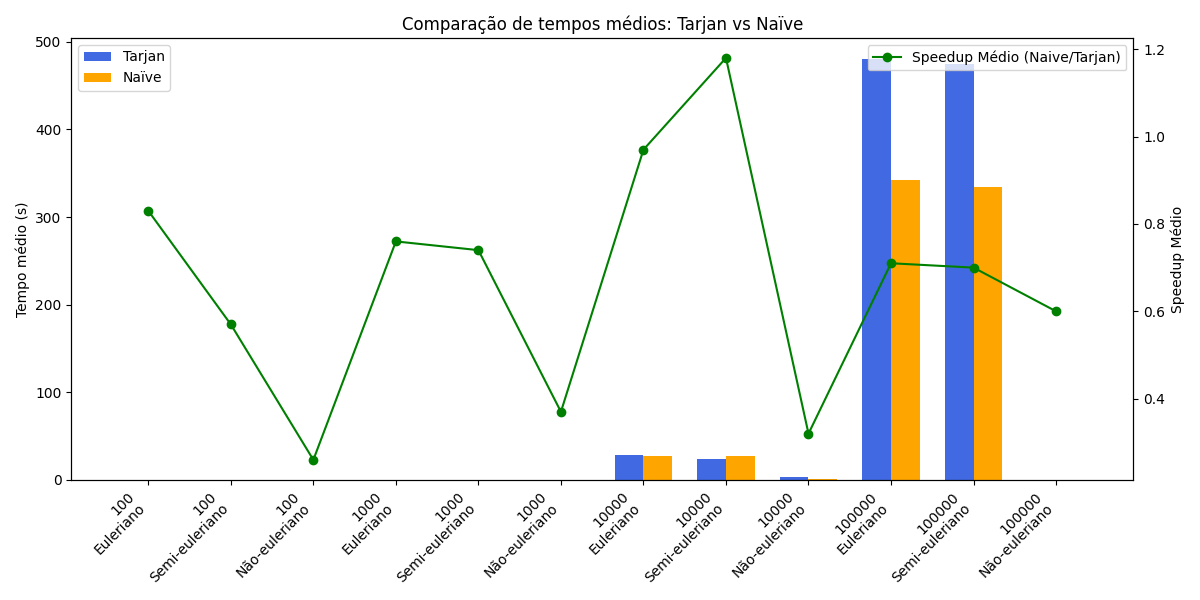
\includegraphics[width=0.9\textwidth]{Figure_1.png}
    \caption{Comparação de tempo}
    \label{fig:Fig1}
\end{figure}

\begin{figure}[H]
    \centering
    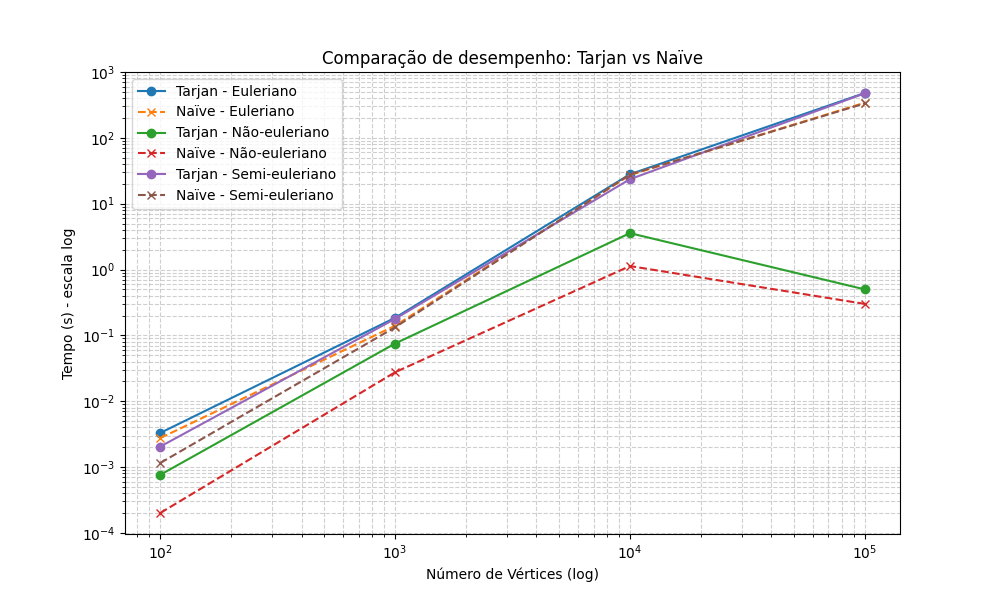
\includegraphics[width=1\textwidth]{Figure_2.png}
    \label{fig:Fig2}
    \caption{Comparação de desempenho}
\end{figure}

\begin{figure}[H]
    \centering
    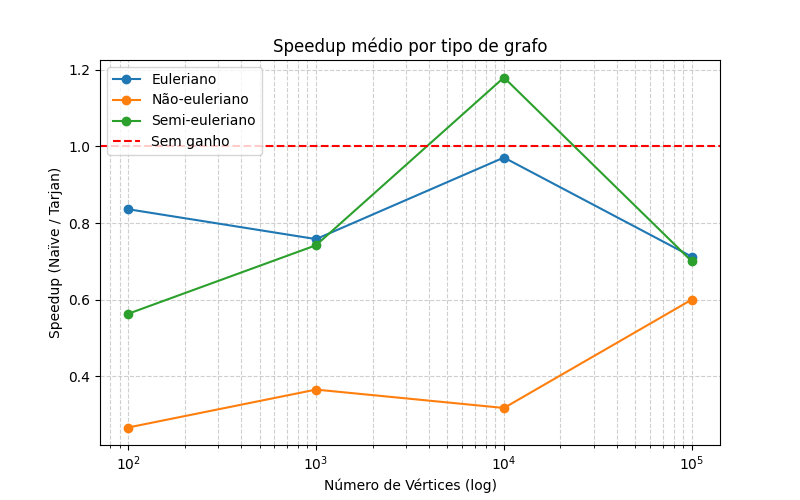
\includegraphics[width=1\textwidth]{Figure_3.png}
    \label{fig:Fig3}
    \caption{Speedup médio}
\end{figure}


\section{Decisões de Implementação}

\subsection{Otimizações Realizadas}

\begin{enumerate}
\item \textbf{Clone de Adjacência}: Uso de HashSet para remoção $O(1)$ de arestas
\item \textbf{DFS Iterativa}: Prevenção de stack overflow em grafos grandes
\item \textbf{Parada Antecipada no Tarjan}: Interrupção da busca ao encontrar a ponte desejada
\item \textbf{Gerenciamento de Memória}: Reutilização de arrays de visitação com marcação por tick
\end{enumerate}

\subsection{Estruturas de Dados Escolhidas}

\begin{itemize}
\item \textbf{Lista de Adjacências}: Eficiente para grafos esparsos
\item \textbf{HashSet}: Remoção rápida de arestas durante execução do Fleury
\item \textbf{ArrayDeque}: Implementação eficiente de pilha para DFS
\end{itemize}

\subsection{Tratamento de Casos Especiais}

\begin{itemize}
\item Grafos desconexos são detectados antes da execução do Fleury
\item Grafos sem arestas retornam lista vazia
\item Validação de propriedades eulerianas antes da construção do caminho
\end{itemize}

\section{Limitações e Trabalhos Futuros}

\subsection{Limitações Atuais}

\begin{enumerate}
\item \textbf{Uso de Memória}: A clonagem do grafo pode ser custosa para grafos muito grandes
\item \textbf{Tipos de Grafo}: Limitado a grafos simples não-direcionados
\end{enumerate}

\subsection{Melhorias Propostas}

\begin{enumerate}
\item \textbf{Algoritmo de Hierholzer}: Implementação mais eficiente para caminhos eulerianos ($O(E)$)
\item \textbf{Detecção Dinâmica de Pontes}: Atualização incremental durante remoção de arestas
\item \textbf{Paralelização}: Exploração de paralelismo na detecção de pontes
\end{enumerate}

\section{Conclusão}

Este trabalho implementou e comparou duas abordagens para detecção de pontes no contexto do algoritmo de Fleury. Contrariamente às expectativas teóricas iniciais, os resultados experimentais revelaram um comportamento surpreendente: o método naïve apresentou performance superior ao algoritmo de Tarjan na maioria dos casos testados.

A análise dos resultados mostrou que o método naïve foi consistentemente mais rápido, com speedups variando de 0,27 a 1,18, indicando que para os tipos de grafos e tamanhos testados, a abordagem simples de contagem de vértices alcançáveis superou a complexidade do algoritmo de Tarjan otimizado. Este comportamento é especialmente notável em grafos não-eulerianos, onde o método naïve demonstrou eficiência significativamente superior.

Várias hipóteses explicam estes resultados inesperados:
\begin{enumerate}
    \item O overhead da implementação do algoritmo de Tarjan com parada antecipada pode não compensar para os tamanhos de grafos testados;
    \item A natureza dos grafos aleatórios gerados pode favorecer a estratégia de contagem simples;
    \item As otimizações específicas na implementação naïve, baseada na referência do GeeksforGeeks, resultaram na melhor eficiência prática.
    \item Apesar do Tarjan ser mais eficiente ao executa-lo separadamente em um grafo, ao utilizar o Fleury, ele precisa ser constantemente chamado pois o grafo se altera na medida em que as arestas sao retiradas
\end{enumerate}

Os resultados demonstram que, embora a análise de complexidade teórica seja fundamental, a performance prática pode divergir significativamente dependendo das características específicas dos dados de entrada e das otimizações de implementação. Para trabalhos futuros, seria interessante explorar implementações alternativas dos algoritmos, bem como testar em tipos específicos de grafos que possam favorecer o algoritmo de Tarjan.

Este relatorio reforça a importância da validação experimental em algoritmos, mesmo quando a teoria sugere um comportamento específico, e destaca que a escolha do algoritmo mais apropriado deve considerar não apenas a complexidade assintótica, mas também as características práticas da implementação e dos dados de entrada.

\nocite{*}
\bibliographystyle{sbc}
\bibliography{sbc-template}

\end{document}